%% This is an example first chapter.  You should put chapter/appendix that you
%% write into a separate file, and add a line \include{yourfilename} to
%% main.tex, where `yourfilename.tex' is the name of the chapter/appendix file.
%% You can process specific files by typing their names in at the 
%% \files=
%% prompt when you run the file main.tex through LaTeX.
\chapter{Conclusions}

With fully reconstructed $B^0_s$ and $B^+$ measurements in PbPb collision, we can study the beauty hadronization mechanism and answer the questions raised in Section 2.7.

\section{$pp$ Reference and Theoretical Models}

Because our fully reconstructed B-meson analysis in $pp$, which serves as the reference for PbPb, is still ongoing, in order to understand our PbPb data, we need to add the B-meson $pp$ measurements from other experiments at the LHC. The $pp$ references we use to compare our PbPb measurement are described below:

\textbf{LHCb 7 TeV pp result at $2 < |y| < 5$:} This reference is chosen because it is one of the most precise $B^0_s/B^+$ measurements with energy is closest to the 5.02 TeV in our analysis \cite{LHCbFF}. The original results are presented as the efficiency corrected yield ratio $\mathcal{R} = \frac{N(B^0_s \rightarrow J/\psi \phi)}{N(B^+ \rightarrow J/\psi K^+)} \cdot \frac{\epsilon(B^+ \rightarrow J/\psi K^+)}{\epsilon(B^0_s \rightarrow J/\psi \phi)}$ \cite{LHCbFF}. We multiply $\mathcal{R}$ by the branching ratios of $BR(B^0_s \rightarrow J/\psi \phi \rightarrow \mu^+\mu^- K^+ K^-)/BR(B^+ \rightarrow J/\psi K^+ \rightarrow \mu^+\mu^- K^+)$ and make them be the same quantity as our $B^0_s/B^+$ measurement.

\textbf{ATLAS 7 TeV pp results at $|y| < 2.5$:} This reference is chosen because it is measured over a rapidity range similar to our measurement range \cite{ATLASPPRef}. The original results are the ratio of the fragmentation fraction $f_s/f_d$. Using the isospin symmetry, we get $f_d = f_u$. So $f_s/f_d = f_s/f_u$. In addition, the ATLAS paper uses the QCD calculation $BF(QCD) = \frac{BR(B^0_s \rightarrow J/\psi \phi)}{BR(B^0 \rightarrow J/\psi K^{*0})} =$ 0.83 instead of directly quoting the PDG the branching ratios $BF(PDG) = \frac{BR(B^0_s \rightarrow J/\psi \phi)}{BR(B^0 \rightarrow J/\psi K^{*0})} =$ 0.85. Hence, we relate ATLAS $f_s/f_d$ to our $B^0_s/B^+$ via $B^0_s/B^+ = BF(PDG)/BF(QCD) \times f_s/f_d$ and compare the ATLAS scaled $pp$ data to our data.


LHCb and ATLAS are measured at different rapidity ranges. However, since the rapidity dependence is not significant in $B^0_s/B^+$ ratio as demonstrated in Figure \ref{BeautyFFLHCb} according to the LHCb publication \cite{LHCbFF}, assuming it is also insignificant in PbPb, we can use the $pp$ reference at different rapidity ranges as references in our $B^0_s/B^+$ measurement.

In addition to the $pp$ references, we also include the theoretical predictions from TAMU (labeled as ``PbPb: TAMU'' in orange) and Cao, Sun, Ko (labeled as ``PbPb: Langevin'' in green) models which have been introduced in Section 1.6. Figure \ref{FinalResults} show the comparison between our $B^0_s/B^+$ measurement with $pp$ references and theoretical model calculations. 

\begin{figure}[hbtp]
\begin{center}
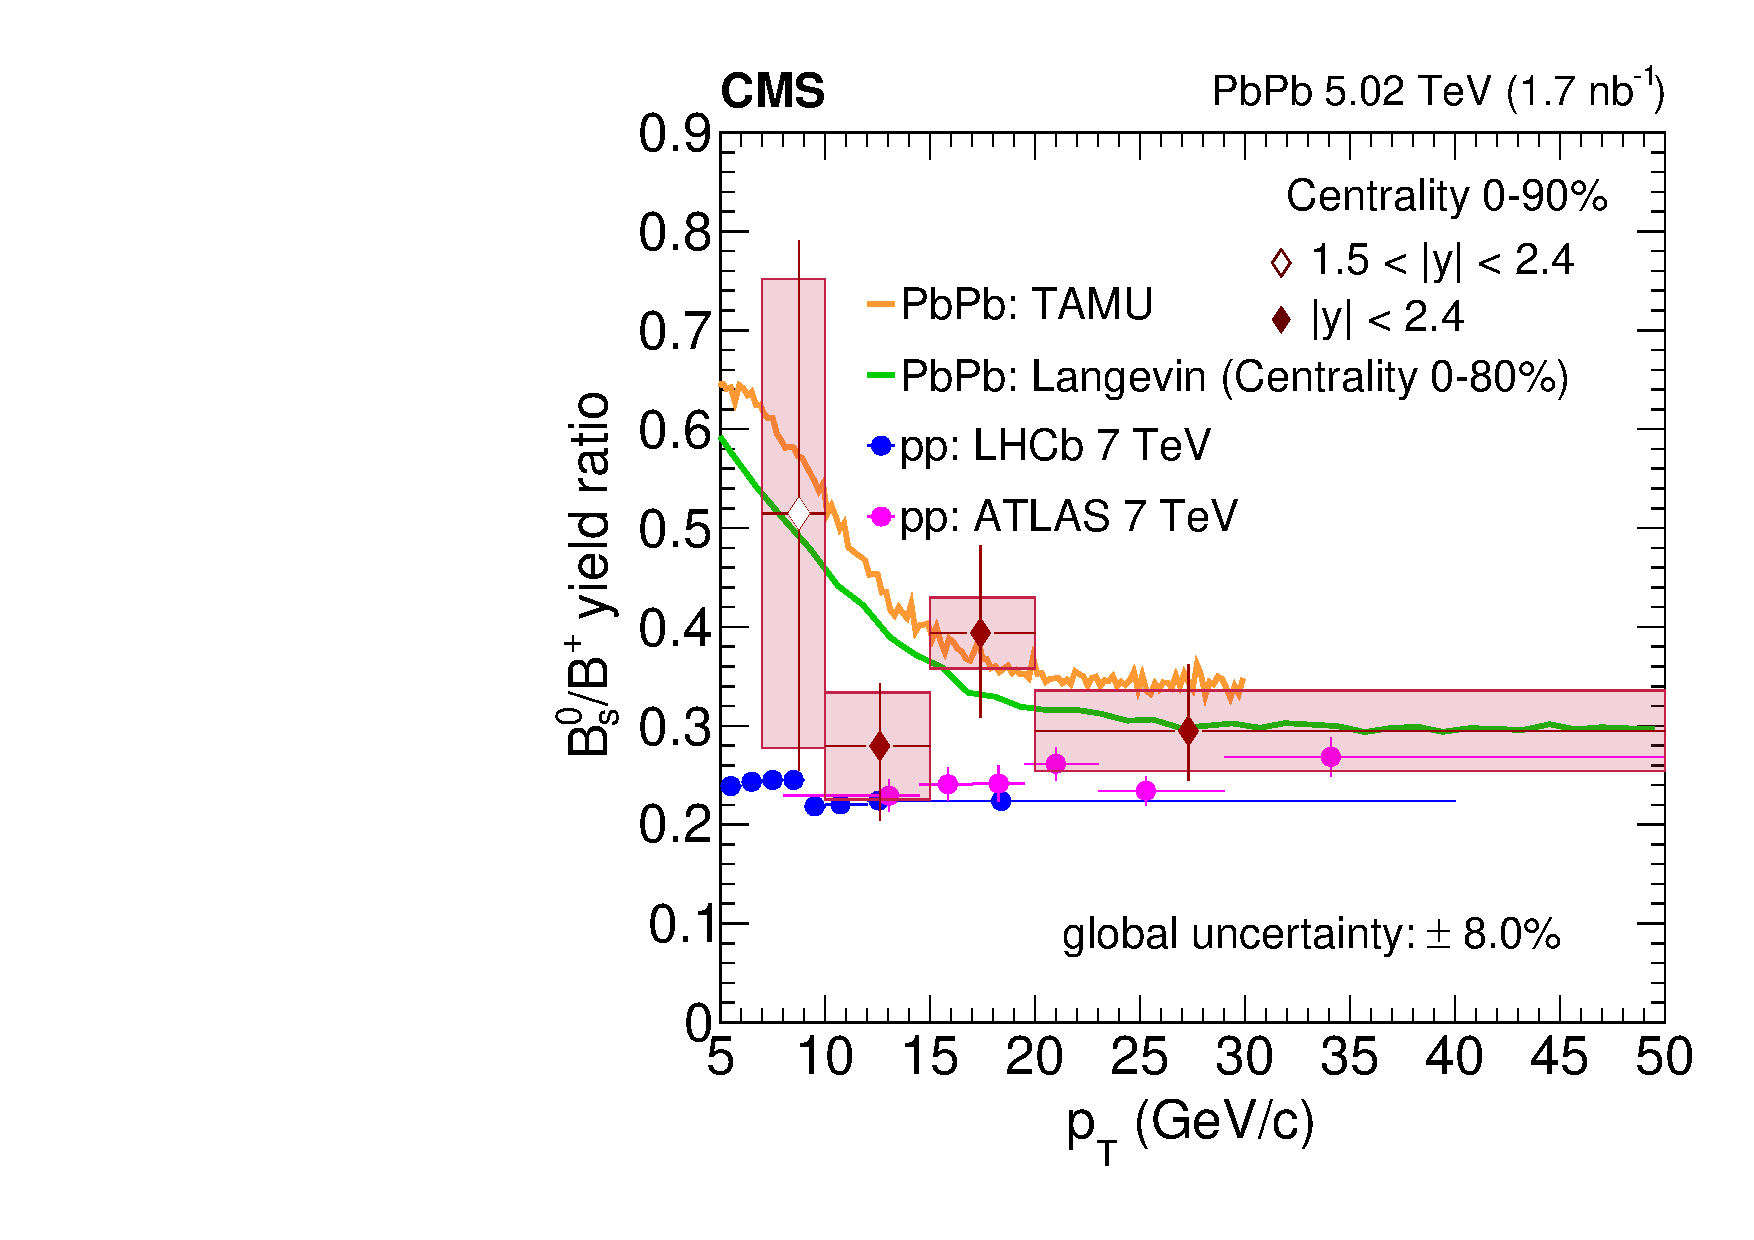
\includegraphics[width=0.48\textwidth]{Figures/Chapter6/ratio_vsPt_ref1_1.pdf}
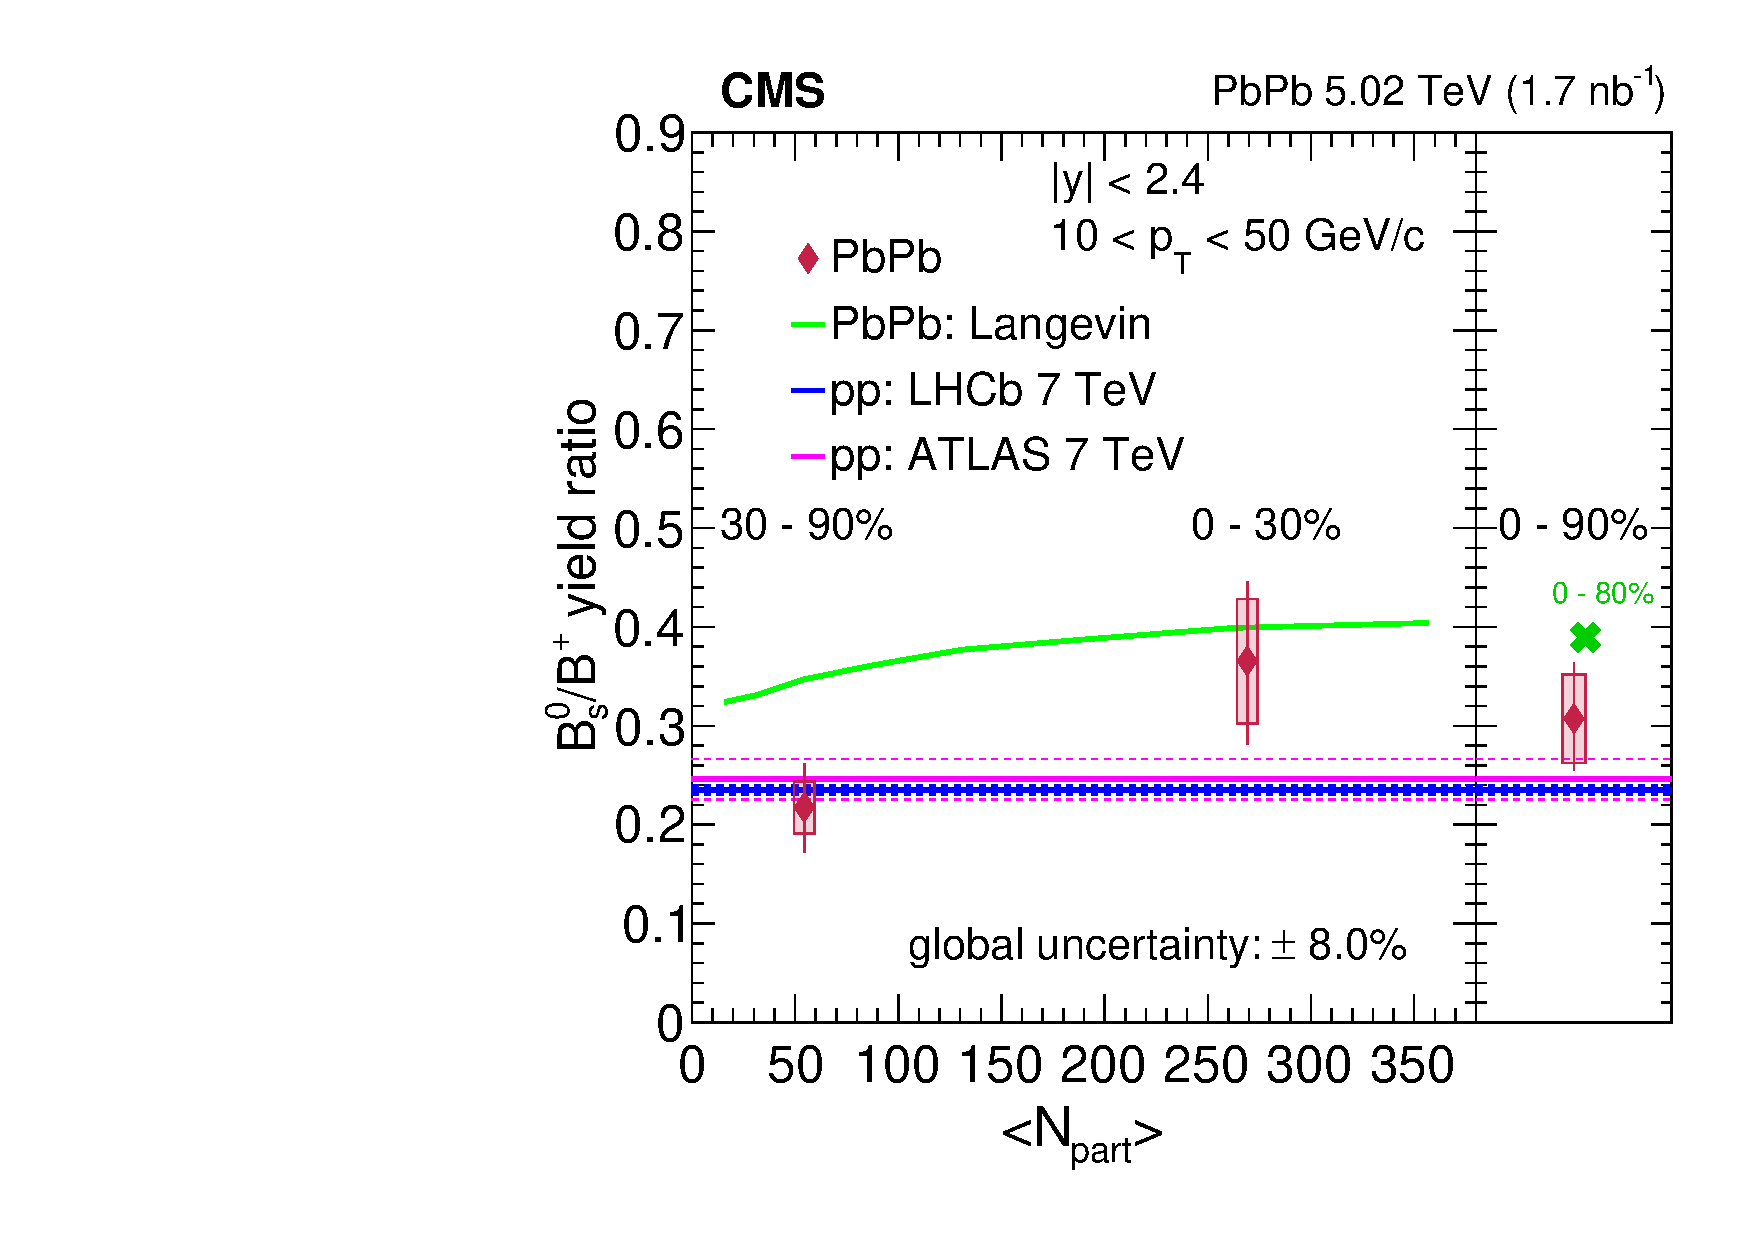
\includegraphics[width=0.48\textwidth]{Figures/Chapter6/ratio_vsCent_ref1.pdf}
\caption{The fully reconstructed $B^0_s/B^+$ (left) and $B^0_s/B^+$ $R_{AA}$ ratio (right) as a function of $p_T$ using the 2015 CMS pp and PbPb datasets are shown above. Both plot include the ATLAS (magenta) and LHCb (blue) 7 TeV $pp$ references. The TAMU model (orange) has only $p_T$ dependent predictions shown on the left figure while the Cao, Sun, Ko model (green) has both $p_T$ and centrality predictions plotted on both figures.}
\label{FinalResults}
\end{center}
\end{figure}   
 

\section{Implications from the Experimental Data}

Figure \ref{FinalResults} conveys a lot of information. We will discuss the physics messages by comparing the PbPb data with the pp references and theoretical model prediction:

%Lies above but with in about 1.5 sigma. not significant $p_T$ dependence. Agree reasonably well with both TAMU and Cao, Sun, Ko models. compatible with LHCb data

%List all the point here

\textbf{Substantial Uncertainties at Low $p_T$:} Both statistical and systematic uncertainties of $B^0_s/B^+$ ratio are large in $7 < p_T < 10$ GeV/c. They all come from $B^0_s$. However, we know that the statistics of $B^0_s$ in the $p_T$ range 7 - 10 GeV/c is indeed very small. In fact, from the FONLL calculation, we expect to get only about 13 $B^0_s$ signal candidates. Unfortunately, some of the systematic uncertainties, for instance, the one due to finite MC simulation statistics, which contributes a lot (26.5\%) to the total systematic uncertainties (46\%) can be in principle further reduced. 

\textbf{No significant $p_T$ dependence:} According to $B^0/B^+$ ratio as a function of B-meson $p_T$, apparently, there is no significant change of the central values for $p_T >$10 GeV/c. For 7 - 10 GeV/c, the central value jumps from 0.28 up to 0.51. However, the uncertainties of the measurement are also very large. Considering all the uncertainties, we do not observe significant $p_T$ dependence on the $B^0_s/B^+$ ratio.

\textbf{Good Agreement with theoretical models:} Comparing the PbPb data to TAMU and Cao, Sun Ko model calculations, the $B^0_s/B^+$ vs $p_T$ data agree well with these two models. They both predict the trend of the central values of our data, which decreases and then approaches flat values as $p_T$ increases. The TAMU model always lies above the Cao, Sun, Ko model because it only employs the quark coalescence model in hadronization. However, in Cao, Sun, Ko model, fragmentation hadronization is also considered. 

However, we know that in the limit $p_T \rightarrow \infty$, the $B^0_s/B^+$ in PbPb collisions will be very similar to $pp$ collisions since the fast-moving beauty quarks traverse through the medium within a very short time and are not likely to combine with any quarks in the medium because they speed are very different. Hence, fragmentation hadronization dominates in b-hadron production at very high $p_T$. 

As for the centrality measurement, the Cao, Sun, Ko model predictions are also reasonably consistent to our in the range of 0 - 30\% and 0 - 90\%. However, in the peripheral 30 - 90\% collisions, the Cao, Sun, Ko model has a lager $B^0_s/B+$ ratio, roughly 2 $\sigma$, compared to our data point, which lies right on the $pp$ references.  


\textbf{Compatible to pp references:} While the centers of $B^0_s/B^+$ data points systematically lie above the $pp$ references, taking into account all uncertainties, they are within about 1 $\sigma$ except the peripheral 30 - 90\% bin with a very small number of participants which behaves like $pp$. However, it should note that the energy of $pp$ reference is higher than the PbPb data. LHCb has reported that the $B^0_s/B^+$ ratio increases as energy goes up \cite{LHCbFF}. Therefore, it would make the comparison much better if we could also perform $B^0_s/B^+$ measurement in $pp$ collisions with CMS and compare it to the PbPb results directly.


%\textbf{Compatible to pp references:}

\section{Conclusions}


With the physics messages obtained from the discussions, we are prepared to answer the questions raised in Section 2.3 and draw conclusions of our studies in this thesis below:



\textbf{First Observation of $B^0_s$ in Nucleus-Nucleus Collisions:} In the analysis, we have fully reconstructed $B^0_s$ with greater 5$\sigma$ significances in all $p_T$ and centrality bins. Therefore, we have improved our measurement compared to the 2015 published results and first observed fully reconstructed $B^0_s$ in heavy-ion collisions.

\textbf{Significant Improvement of the Previous Results:} We have successfully reproduced the published results using 2015 datasets with higher precision. Moreover, our new results measure $B^0_s/B^+$ as a function of centrality for the first time. In addition, thanks to the higher statistics of the dataset, we are able to measure four $p_T$ bin, providing more information about the $p_T$ dependence of the $B^0_s/B^+$ ratio. In our measurement, we find no significant $p_T$ dependence of $B^0_s/B^+$ down to at least 10 GeV/c. In addition, there is a hint of suppression of B-meson cross section in central collision compare to peripheral collisions, which will be confirmed with larger statistics later. 
 
\textbf{Inconclusive about Strangeness Enhancement:} There is a weak hint of potential strangeness enhancement for beauty quark hadronization in PbPb collisions, particularly at low $p_T$, compared to $pp$ collisions. The $B^0_s/B^+$ ratios in PbPb are systematically higher than pp with about 1 - 1.3 $\sigma$. However, the hint is not strong enough. We will need more statistics to confirm this hint in the future.

\textbf{The fragmentation hadronization mechanism alone is not enough to describe our data:} We can see that the quark coalescence effect must be considered because our data points lie systematically above the $pp$ references. Looking at the most central collision from 0 - 30 \%, the $B^0_s/B^+$ ratio is about 1.25$\sigma$, which corresponds to about 80\% confidence, above the LHCb pp reference. The explicit computation is shown as follows:

\begin{equation}
\% Dev = (0.3655 - 0.2353)/(0.3655 * \sqrt{0.23^2 + 0.172^2}) \simeq 1.25 
\end{equation}


\textbf{Not Enough Precision to Constrain Theoretical Models:} Base on the uncertainties of our data, we find that the theoretical models using quark coalescence as hadronization model, for instance, the TAMU and Cao, Sun, Ko models, are all in reasonable agreement with the PbPb data, both in terms of central values and the decreasing trends as $p_T$ increases.

\textbf{Missing B-meson Measurement in $pp$ with CMS as A Reference:} Currently, the B-meson $pp$ analysis is still working in progress. More results will be coming in the near future to answer the questions such as beauty energy loss mechanism in the QGP and hadronization mechanism in small systems. Our B-meson $R_{AA}$ measurements will be able to constrain the heavy-quark spatial diffusion coefficient and the jet transport parameter to probe the inner workings of the QGP.

In conclusion, the larger PbPb datasets that should be accumulated in upcoming LHC Run 3 and high-luminosity (HL) LHC heavy-ion runs will provide greater precision and allow more differential B-meson measurements not only on traditional observables with but also on modern observables such as $B-\bar B$ angular correlations with more fully reconstructed b-hadron species such as $\Lambda_b$, $B^0_c$, and $\Omega_b$. In addition, the CMS MIP Timing Detector (MTD) upgrade \cite{CMSMTD} will allow us to perform hadronic PID. We will be able to fully reconstruct beauty hadrons down very low $p_T$ and carry out measurements with high precision. These future b-hadron measurements could help further investigate beauty hadronization in vacuum and QGP.


%The $B^0_s$ and $B^+$ mesons are studied with the CMS detector at the LHC via the reconstruction of the exclusive hadronic decay channels B\ and \Bplusdecayall.  The measurements are performed within the \PB\ mesons' fiducial region given by transverse momentum $\pt>10\GeVc$ for rapidity $\abs{y}<1.5$  and  $7<\pt<50\GeVc \,$ for $1.5<\abs{y}<2.4$. The first observation of the \PBzs\ meson in nucleus-nucleus collisions, with a statistical significance well surpassing five standard deviations, is attained. The production yields of \PBzs\ and \PBp\ mesons, scaled by the nuclear overlap function \TAA and the number of minimum bias events \NMB, in lead-lead (\PbPb) collisions at a center-of-mass energy of $5.02\TeV$ per nucleon pair are presented as functions of the meson \pt\ and for the first time of the event centrality. These results extend, and are compatible with, those previously reported by the CMS Collaboration~\cite{BsPbPbCMS,BpPbPbCMS}, and are based on a three-fold larger \PbPb\ data sample. The ratio of production yields of the two mesons in \PbPb\ collisions is determined and it is found to be statistically compatible with the corresponding ratio in proton-proton (\pp) collisions. The further investigation of possible hints of an enhancement of the ratio in \PbPb, relative to \pp, collisions will benefit from more precise \PbPb\ and \pp\ reference data taken at the same collision energy per nucleon. The larger \PbPb\ data sets that should be accumulated in upcoming high-luminosity LHC heavy ion runs will provide greater precision and could help to further characterize the mechanisms of beauty hadronization in heavy ion collisions.






%We have performed the 
%Conclude the message. Draw final based on the points. Answer question post previously

%More precise measurement. 



\section{Future Outlooks}

As mentioned previously, our $pp$ data analysis is still ongoing. Figure \ref{BPLow}, Figure \ref{BZLow}, and Figure \ref{BsLow} show our ongoing analysis of fully reconstructed $B^0_s$, $B^+$, and $B^0$ using the 2017 $pp$ datasets at $\sqrt {s_{NN}} = $ 5.02 TeV at very low $p_T$ respectfully.


\begin{figure}[hbtp]
\begin{center}
\includegraphics[width=0.60\textwidth]{Figures/Chapter6/BPLow.pdf}
\caption{The fully reconstructed $B^+$ via the decay channel of $B^+\rightarrow J/\psi K^+ \rightarrow \mu^+\mu^- K^+$ in the $p_T$ range of 0 - 1 GeV/c using the full CMS 2017 $pp$ dataset is shown above. The statistical significance is about 6. The selection is optimized with the BDT algorithm using a subset of topological variables used in PbPb $B^+$ studies.}
\label{BPLow}
\end{center}
\end{figure}   
 
 \begin{figure}[hbtp]
\begin{center}
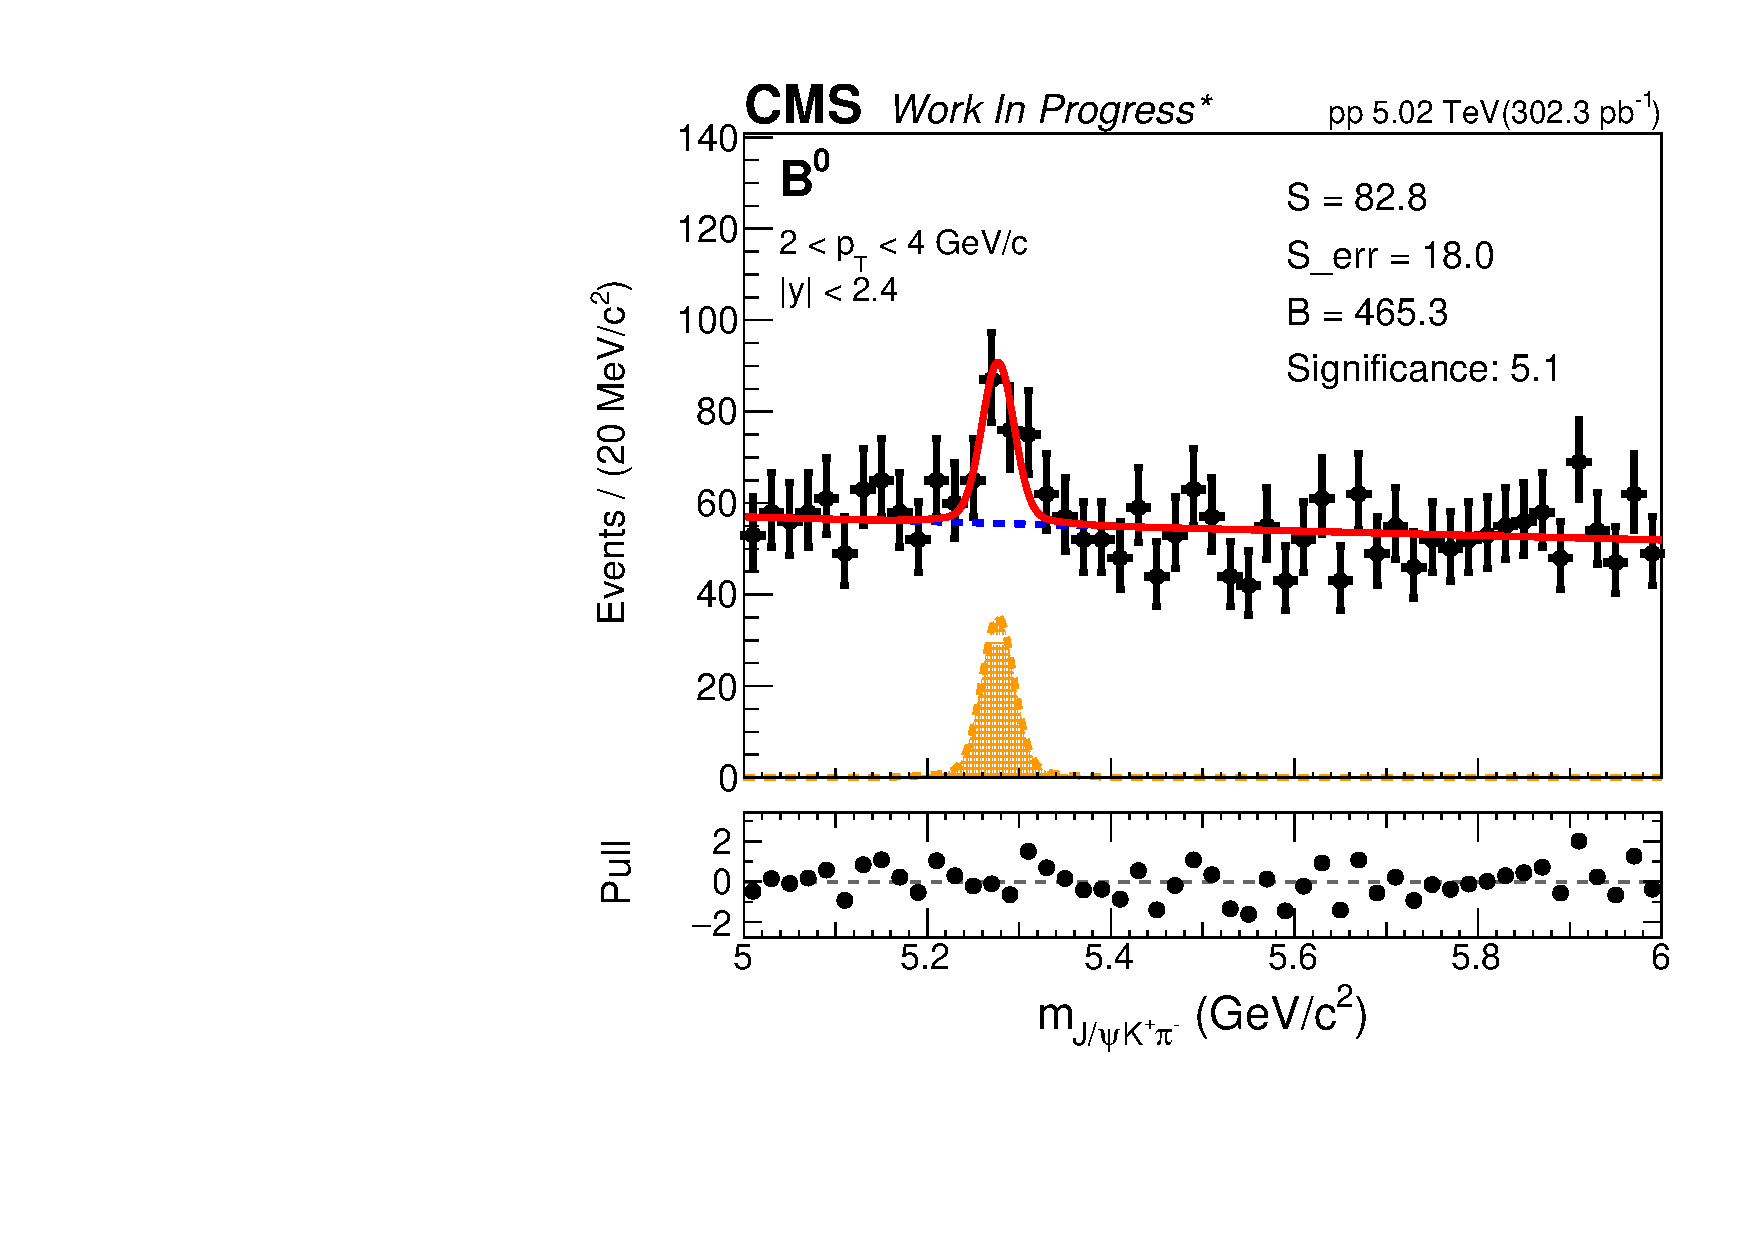
\includegraphics[width=0.60\textwidth]{Figures/Chapter6/BZLow.pdf}
\caption{The fully reconstructed $B^0$ via the decay channel of $B^0\rightarrow J/\psi K^{0*} \rightarrow \mu^+\mu^- K \pi$ in the $p_T$ range of 2 - 4 GeV/c using the full CMS 2017 $pp$ dataset is shown above. The statistical significance is about 5.1. The selection is optimized with the BDT algorithm using a subset of topological variables used in PbPb $B^0_s$ studies.}
\label{BZLow}
\end{center}
\end{figure}   

 \begin{figure}[hbtp]
\begin{center}
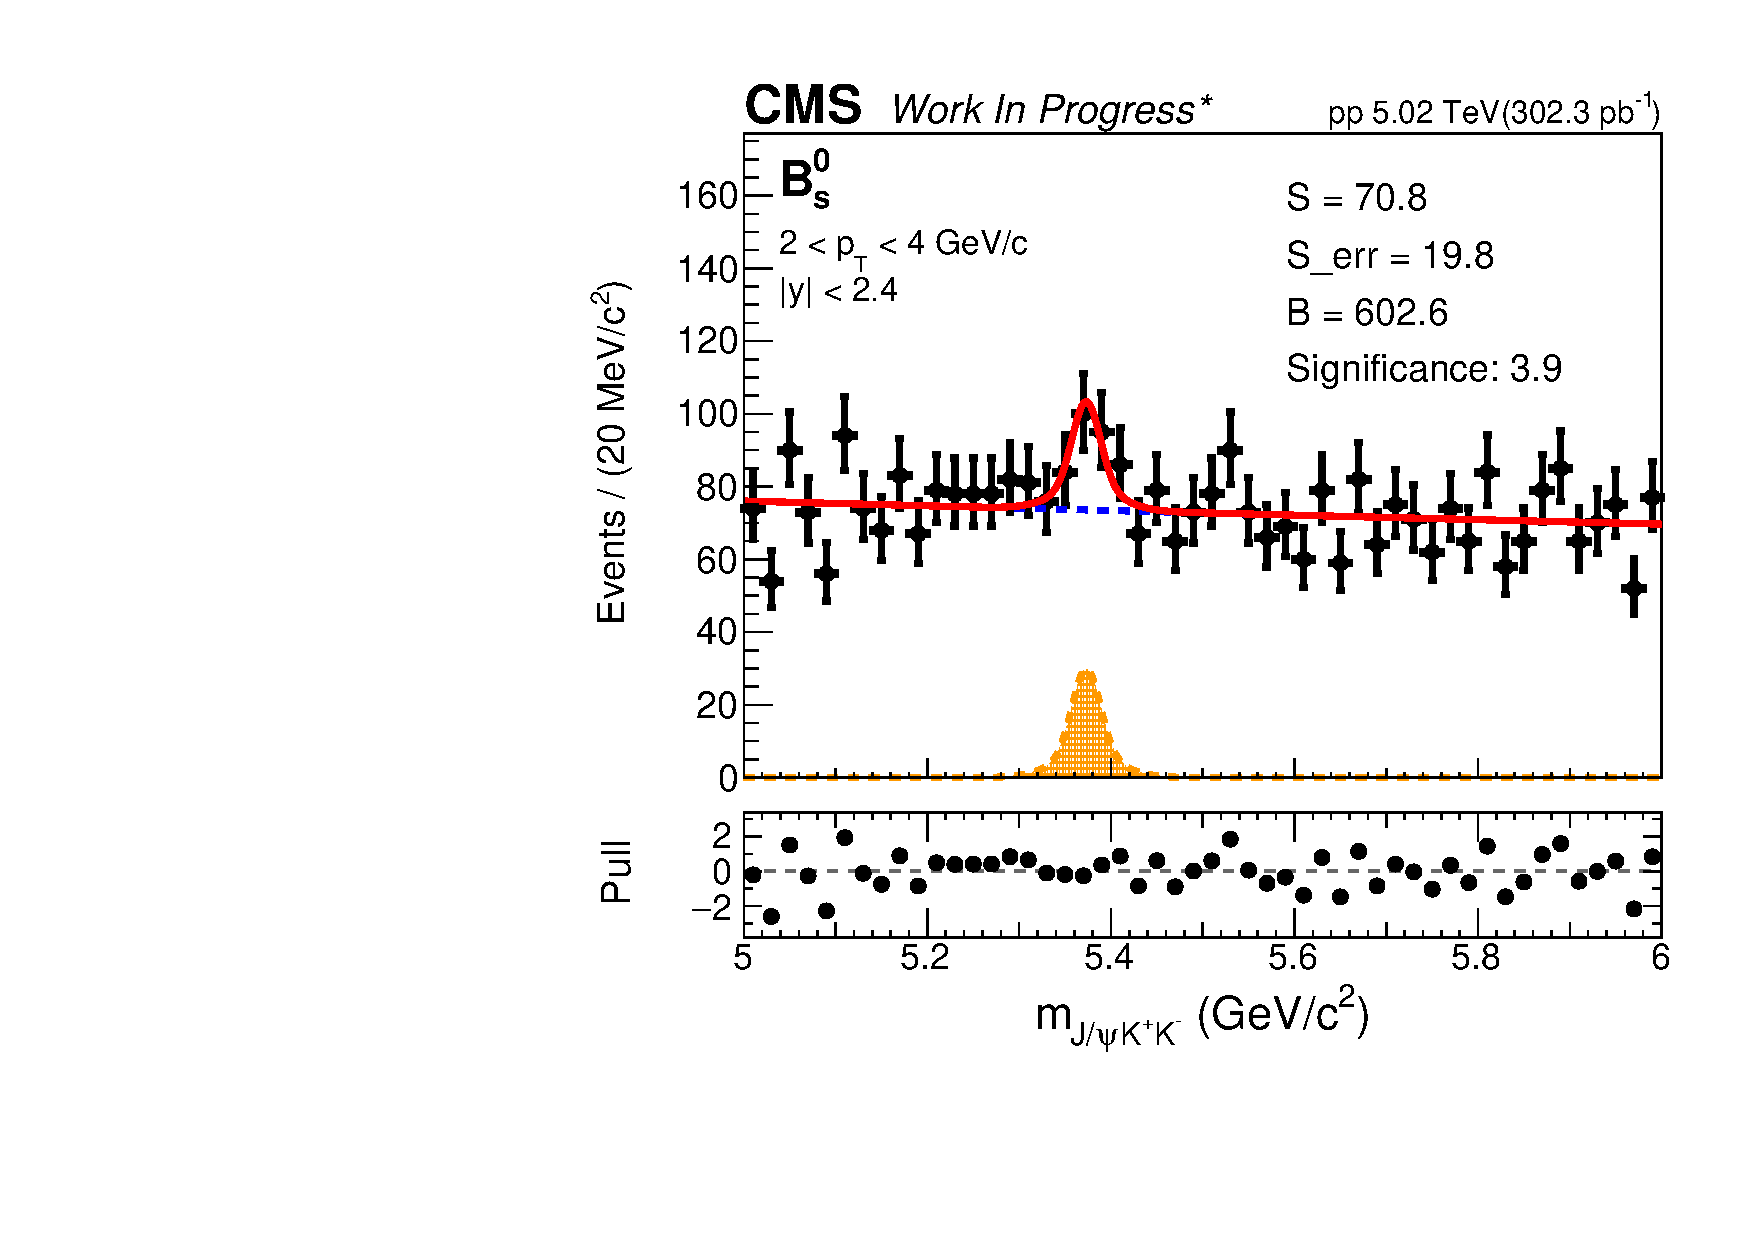
\includegraphics[width=0.60\textwidth]{Figures/Chapter6/BsLow.pdf}
\caption{The fully reconstructed $B^0_s$ via the decay channel of $B^0_s\rightarrow J/\psi \phi  \rightarrow \mu^+\mu^- K^+ K^-$ in the $p_T$ range of 2 - 4 GeV/c using the full CMS 2017 $pp$ dataset is shown above. The statistical significance is about 3.9. The selection is optimized with the BDT algorithm using a subset of topological variables used in PbPb $B^0_s$ studies.}
\label{BsLow}
\end{center}
\end{figure}   

Thanks to the powerful machine learning algorithms, even without hadronic PID, very clear B-meson signals have still been observed down to $p_T =$ 0. The estimated significances are all greater than 4. With these significant signals, we can perform precise measurement on $B^+$ cross section in $pp$ collisions down to $p_T =$ 0, which allows us to study inclusive beauty production cross section. In addition, we will also be able to measure $B^0_s/B^+$ ratio down to 2 GeV/c. Finally, according to the multiplicity studies, we can also $B^0_s/B^+$ as a function of multiplicity up to about 150, which helps us answer many questions raised in Chapter 2.  These fully B-meson measurements down to very low $p_T$ and up to very high multiplicity will shed light on the beauty quark hadronization mechanisms in vacuum and QGP.

In the future era of LHC Run 3 and HL-LHC, much more data will be collected to perform exciting measurements on fully reconstructed $B^+_c$ and $\Lambda_b$ hadrons. Finally, at RHIC, as the sPHENIX experiment is taking data in 2023, we can also fully reconstruct b hadrons at lower energies to study a QGP medium at lower temperatures and higher baryon chemical potentials. The fully reconstructed b-hadron measurement at RHIC will be complementary to the measurements at the LHC. Together, these will help determine the heavy-quark diffusion coefficient at different temperatures, constrain the fundamental property of QGP $\eta/s$, and probe the inner workings of QGP. Lots of challenges and opportunities are waiting for us to explore and overcome. A bright and exciting chapter of relativistic heavy-ion physics is forthcoming in the near future.



